% Nature Communications manuscript, v2 reorganised 2026-11-26 around the published-methods test (PREREG_EXTERNAL.md) and the forced-answer amendment (PREREG_MATH4500_AMEND1.md),
% the 32k / forced-answer / control runs (synth/natcomm_32k_analysis.py -> ../data/natcomm_32k.json) and
% synth/natcomm_conf_analysis.py -> ../data/conf4500_result.json. Exploratory MATH-500 8k numbers as in v1 (paper_stats.json).
\documentclass[10pt]{article}
\usepackage[a4paper,margin=2.05cm,top=2.2cm,bottom=2.2cm]{geometry}
\usepackage[T1]{fontenc}
\usepackage{mathptmx}
\usepackage{helvet}
\usepackage{graphicx,amsmath,xcolor,float,setspace,titlesec,caption,booktabs,needspace,upquote}
\usepackage[super,comma,sort&compress]{natbib}
\usepackage[hidelinks]{hyperref}
\usepackage{xr-hyper}
\externaldocument[S-]{si_v2}
\newcommand{\sref}[1]{\ref{S-#1}}
\definecolor{ncteal}{HTML}{1B7F6E}
\bibliographystyle{naturemag}
\setstretch{1.12}
\widowpenalty=10000\clubpenalty=10000% no single line of a paragraph alone at the top or bottom of a page
\captionsetup{font=small,labelfont=bf,labelsep=period}
\renewcommand{\topfraction}{0.8}\renewcommand{\textfraction}{0.15}
% keep every heading with its rule and the first lines of its text
\titleformat{\section}{\Needspace{6\baselineskip}\sffamily\bfseries\large\color{ncteal}}{}{0pt}{}[\nopagebreak\vspace{1pt}\color{ncteal}\titlerule\vspace{2pt}]
\titlespacing{\section}{0pt}{11pt}{4pt}
\titleformat{\subsection}{\Needspace{4\baselineskip}\sffamily\bfseries\normalsize}{}{0pt}{}
\titlespacing{\subsection}{0pt}{8pt}{3pt}
\graphicspath{{../figures/}}
\newcommand{\E}{\mathrm{E}}

\title{\sffamily\bfseries\Large Does shorter reasoning mean better reasoning?}
\author{\normalfont Cristiano Capone\\[2pt]\normalsize Quantitative Health Models and Bioinspired Technologies Lab, Istituto Superiore di Sanit\`a, Rome, Italy\\[1pt]\small\texttt{cristiano.capone@iss.it}}
\date{}

\begin{document}
\maketitle
\suppressfloats[t]

\begin{abstract}
\noindent Language models trained to reason briefly often gain accuracy by finishing within a token limit. How much can their starting models recover when prompted to conclude? In a pre-registered test on MATH-500, four length-reduction methods gained 10.1 percentage points on average when unfinished attempts scored zero. Forcing unfinished attempts from both models to answer reduced the gain to 1.0 point while the methods used 40--55\% fewer tokens. We then varied which of its own verified solutions a model learned from. On 4,500 held-out problems, shortest replay gained 1.04 points over random replay. With forced answers it retained 0.34 points at 5.4\% fewer tokens. On problems eliciting both short and long responses from the starting model, long attempts fell from 49\% under random selection to 30\% under shortest selection (exploratory). Shorter reasoning thus mostly meant finishing sooner rather than reasoning better, and choosing among correct examples can teach it.
\end{abstract}

\section{Introduction}
Language models that reason before answering spend most of their compute on the reasoning itself, and they run under a cap on the tokens they may generate. Longer reasoning is not monotonically better: models overthink easy inputs\cite{chen2024overthinking} and, as agents, deliberate when they should act\cite{cuadron2025overthinking}. Reasoning can be shortened by prompting\cite{xu2025chainofdraft}, by controlling the budget at test time\cite{muennighoff2025s1,ma2025nothinking,xu2026elastic,qi2025anytime}, by fine-tuning on concise self-generated traces\cite{munkhbat2025concise} or by reinforcement learning with length-aware rewards or a hard token limit\cite{yi2025shorterbetter,hou2025thinkprune,aggarwal2025l1,shrivastava2026gfpo,liu2025dler} (reviewed in ref.~\citenum{sui2025stopoverthinking}). In parallel, models are improved by training on their own verified outputs: self-taught reasoning\cite{zelikman2022star}, rejection-sampling fine-tuning\cite{yuan2023rft} and reinforced self-training\cite{gulcehre2023rest}. In all three, every verified solution is an equally good target. Many length-reduction methods report higher accuracy as well as shorter reasoning. Under a limit on generated tokens such a gain can mean two different things: the model reasons better, or more of its attempts end before the limit while the others are cut and scored as wrong.

Keeping the shortest verified solution is a known heuristic. Kimi k1.5 fine-tunes on the shortest of several correct samples\cite{kimi2025k15}, thinking-optimal scaling selects it for self-improvement\cite{yang2025tops}, and fine-tuning on it shortens reasoning at roughly unchanged accuracy\cite{munkhbat2025concise,chen2024overthinking}. Hassid and colleagues fine-tuned models on the shortest, a random or the longest of several chains written by another model and found the shortest best for a 32-billion-parameter student but not consistently for a 7-billion-parameter one\cite{hassid2025overthink}. Recent analyses decomposed reasoning efficiency or accuracy under a budget into completing within it and being correct when complete\cite{kaiser2026decomposing,nie2026truncation}, found that concise reasoning helps mainly by finishing before the deadline and recommended reporting the answer obtained when a run is stopped\cite{carlon2026shorter}, charged the final answer to the same budget as the reasoning\cite{chang2026answer}, and found that released reinforcement-learning models gain mostly by finishing at 4k and 8k tokens\cite{yang2026outcome}. What has not been done is to re-evaluate published length-reduction methods under a pre-registered protocol, with a forced answer as the counterfactual, and to manipulate, with matched controls, which of a model's own verified solutions it is trained on.

These mechanisms are not exclusive, and we separate them with a forced answer: when the budget runs out, the reasoning is closed and the model is asked to answer\cite{qwen3report,muennighoff2025s1}. A method whose attempts only stop earlier gains nothing over a starting model that is forced to answer; one that progresses faster keeps a gain at tight limits, and one that reasons better keeps it at any limit (Fig.~\ref{fig:concept}). We apply this test to published methods and to matched controls: identical copies of a model fine-tuned on the shortest (S), a random (R) or the longest (L) of its own verified solutions to the same problems, with the same answers and recipe, against the untouched model. We read the results through one idea. If an attempt needs $L$ tokens to reach its answer and the cap is $t$, attempts that do not finish are lost, and the cap acts as a restart cutoff in the sense of Luby, Sinclair and Zuckerman\cite{luby1993optimal}. Replaying short solutions should shift $L$ to the left without changing which answers the model can reach. Its benefit should then appear in the share of attempts that finish, not in the correctness of the answers that finish; it should disappear when the cap stops binding; and the shorter policy should stay cheaper.

The results are these. Three published methods that shorten reasoning by reinforcement learning gained 13.8 points over their common starting model at 4k and 8k tokens when cut attempts were scored as wrong and 3.1 points with forced answers (pre-registered), about half of it matching a descriptive model of faster progress and the rest from DLER; what remained was a saving of 40--55\% in tokens. In our controlled experiment, the shortest-replay model beat the random-replay model on 4,500 held-out problems through finishing (pre-registered); the ordering S $>$ R $>$ L held, in point estimates, across training runs, model families and programming, and we found no evidence that it reflects training dose, the pipeline or sharpening. A forced answer removed two-thirds of the advantage, leaving 0.34 points, close to a descriptive model of faster progress, at about 5\% fewer tokens. Shorter reasoning thus finished more often, progressed somewhat faster and cost less; it gave better answers only where the training itself improved them.

\begin{figure}[t]
\centering
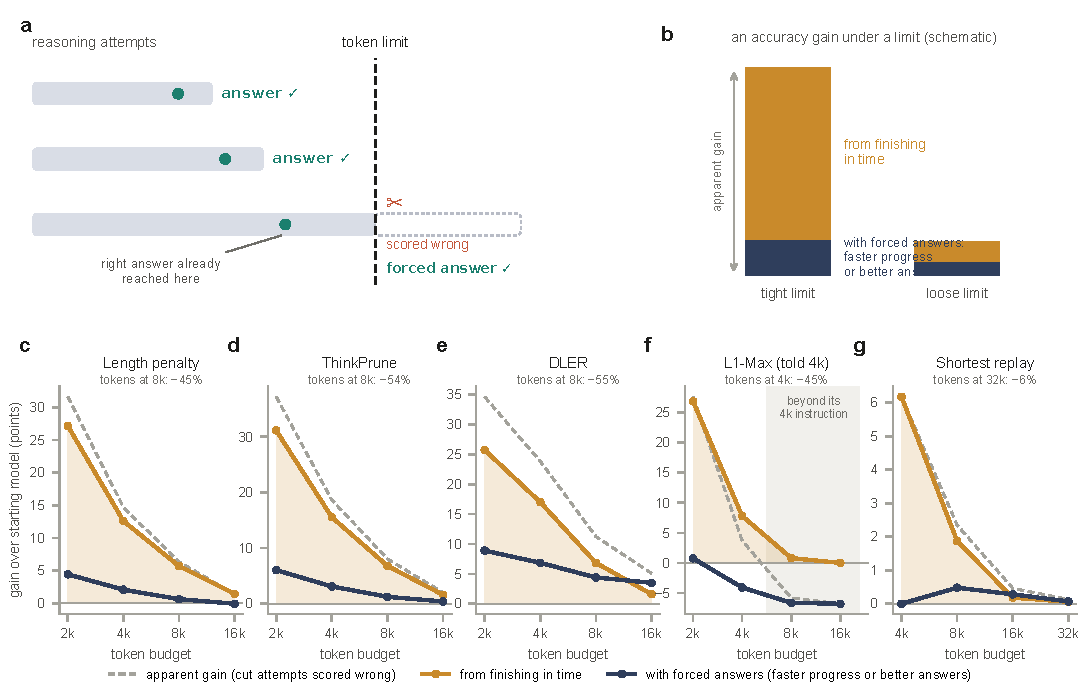
\includegraphics[width=\textwidth]{fig_split.pdf}
\caption{\textbf{Where an accuracy gain under a token limit comes from.} \textbf{a}, Reasoning attempts against a token limit (schematic): an attempt that reaches the limit is cut; scored as wrong, it counts as a failure even when its reasoning had already reached the right answer, which a forced answer at the limit recovers. \textbf{b}, The apparent gain of a method over its starting model, with cut attempts scored as wrong, splits into the part that disappears when both are forced to answer at the limit (from finishing in time) and the part that remains (with forced answers), which includes faster progress as well as better answers; both shrink as the limit loosens (schematic). \textbf{c}--\textbf{g}, The two parts measured against the token budget on MATH-500, for four published methods against their starting models (16k generations; budgets of 4k and 8k pre-registered) and for shortest replay against the untouched Qwen3-4B (32k generations; exploratory). Vertical scales differ between panels. Labels give the change in generated tokens, forced answers counted (at 4k for L1-Max; at 32k for shortest replay). Shaded in \textbf{f}, budgets beyond the 4k that L1-Max was told.}
\label{fig:concept}
\end{figure}

\section{Results}
\subsection{Where the gain comes from, and how reasoning is shortened}
Figure~\ref{fig:concept}c--g splits each gain into the part from finishing in time, which disappears when the starting model is also forced to answer, and the part that survives a forced answer, as a function of the token budget. The first dominates at tight budgets and fades as the budget grows. The second is not, by itself, a gain in the answers: a method that progresses faster is further along when it is cut. For the length penalty, ThinkPrune and shortest replay it is close to a descriptive model of faster progress, the starting model's forced accuracy at the budget divided by the ratio of median lengths (Supplementary Note~8); DLER kept more and L1-Max, at the budget it was told, less. The methods shorten reasoning in three ways (Fig.~\ref{fig:phase}). A length penalty rescales the distribution of reasoning lengths: the starting model's lengths, multiplied by one factor, approximately predict the share of attempts finished (Fig.~\ref{fig:phase}a,f). Methods trained with a hard length limit (ThinkPrune, DLER, L1-Max and DeepScaleR) cut its tail (Fig.~\ref{fig:phase}b,d). The untouched Qwen3-4B solves most problems either in about 1{,}500 or in about 8{,}000 tokens; on the quarter of problems where it does both, shortest replay lowered the share of long attempts to 30\%, against 49\% under random replay ($-18.5$ points, $-22$ to $-15$), and the length of each path stayed the same (Fig.~\ref{fig:phase}c,e). With few methods per regime, the way of shortening and the gain show no simple relation (Fig.~\ref{fig:phase}d).

\begin{figure}[t]
\centering
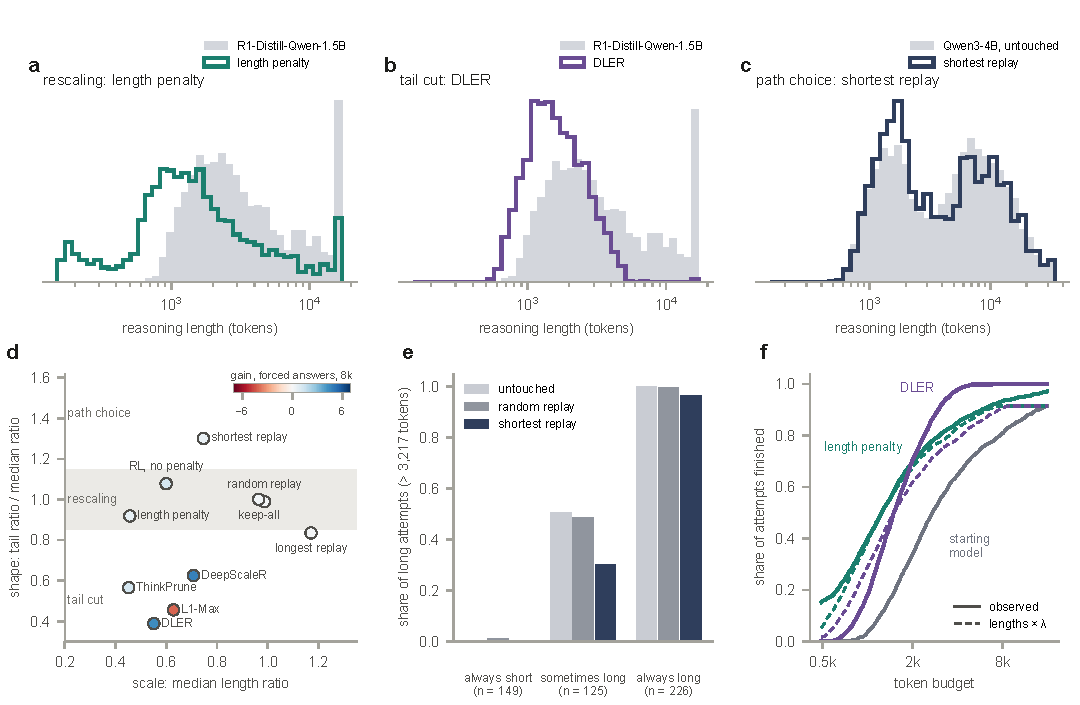
\includegraphics[width=\textwidth]{fig_mechanisms.pdf}
\caption{\textbf{Three ways of shortening reasoning (exploratory).} \textbf{a}--\textbf{c}, Distribution of reasoning lengths of a method (line) and of its starting model (grey): a length penalty rescales it, apart from a group of very short attempts (\textbf{a}), DLER cuts its tail (\textbf{b}), and shortest replay moves attempts from a long to a short path (\textbf{c}; Qwen3-4B, 32k generations). \textbf{d}, Every model by scale, the ratio of its median length to that of its starting model, and shape, the ratio of the 90th percentiles divided by the ratio of the medians (1, rescaling; below 1, tail cut; above 1, path choice); colour, gain with forced answers at 8k (L1-Max at the 4k budget it was told). Published methods are compared with R1-Distill-Qwen-1.5B (L1-Max with DeepScaleR-1.5B), the replay arms with the untouched Qwen3-4B; with 16k generations 8.5\% of R1-Distill-Qwen-1.5B's attempts are cut, which lowers its 90th percentile and so the shape of the published methods. \textbf{e}, Share of long attempts (over 3{,}217 tokens, the valley between the two paths) on the problems that the untouched model, in 8 attempts, always solved short, sometimes long or always long (the untouched model's bars in the outer groups are 0 and 1 by construction; compare shortest with random replay). \textbf{f}, Share of attempts finished within each budget (solid) and the prediction for a method that only rescales length, the starting model's lengths multiplied by the ratio of the medians (dashed); the prediction cannot extend beyond the starting model's 16k cap, so it levels off at its finished share.}
\label{fig:phase}
\end{figure}

\subsection{Published length-reduction methods gain mostly by finishing (pre-registered)}
We first re-evaluated four published methods that shorten reasoning by reinforcement learning, in a pre-registered test (Fig.~\ref{fig:ext}a--d; Methods; Supplementary Note~5). Three start from DeepSeek-R1-Distill-Qwen-1.5B\cite{guo2025deepseekr1}: a length penalty with weight $\alpha=0.2$ (Arora and Zanette\cite{arora2025training}), ThinkPrune\cite{hou2025thinkprune} and DLER\cite{liu2025dler}; the fourth, L1-Max\cite{aggarwal2025l1}, starts from DeepScaleR-1.5B-Preview (\texttt{agentica-org/DeepScaleR-1.5B-Preview}) and was told a budget of 4{,}096 tokens. We generated four samples per MATH-500 problem from each method and its starting model with a 16k-token cap, and forced answers at budgets of 1k to 16k tokens (Methods). The hypothesis was that, at the budgets of 4k and 8k tokens, each method's accuracy gain over its starting model is smaller with forced answers than with cut samples scored as wrong.

It was supported. Averaged over the four methods and the two budgets, the gain was 10.1 points with cut samples scored as wrong and 1.0 point with forced answers, a difference of $-9.1$ points (95\% CI $-10.5$ to $-7.9$; $P<2\times10^{-4}$); in each of the eight method--budget cells the difference was negative with an interval excluding 0. For the three methods that start from R1-Distill-Qwen-1.5B the gain fell from 13.8 to 3.1 points; L1-Max, told a budget of 4{,}096 tokens, is compared at 8k with a starting model that may reason for 8k tokens, which favours the starting model in that cell. With cut samples scored as wrong the length penalty, ThinkPrune and DLER were 14.7, 18.7 and 23.9 points ahead of their starting model at 4k. With forced answers the same methods were 2.1, 3.1 and 6.9 points ahead at 4k and 0.7, 1.3 and 4.4 points at 8k, where only DLER's gain excluded 0 (2.7 to 6.2); DLER kept 3.5 points at 16k (1.8 to 5.3), a gain that forcing does not explain; DeepScaleR, trained by reinforcement learning from the same starting model without a length penalty in its reward (though with staged context limits), reached the same accuracy (84.8\% against DLER's 84.2\% at 16k with forced answers; exploratory, each with its own prompt), so this gain more likely comes from the reinforcement learning than from the length penalty. L1-Max, told a budget of 4{,}096 tokens, used about a third of it (median 1{,}240 tokens); at that budget it was 3.7 points ahead of DeepScaleR with cut samples scored as wrong and 4.1 points behind with forced answers ($-5.8$ to $-2.5$). Looser budgets, which its instruction forbade, are not informative. Against the same reinforcement learning without the penalty, the length penalty gained 3.1 points at 4k with cut samples scored as wrong and 0.3 ($-1.2$ to 1.7) with forced answers. What remained was cost: counting the forced answers, the four methods generated 40--45\% fewer tokens than their starting models at 4k and 45--55\% fewer at 8k (Supplementary Table~\sref{tab:ext}).

At equal average spending rather than at a nominal budget, the question of a service that pays for its tokens, the three methods sharing a starting model were more accurate at every cost they cover (Fig.~\ref{fig:ext}e--g; exploratory, unpaired); L1-Max spent fewer tokens than DeepScaleR at every budget, so they share no cost (Fig.~\ref{fig:ext}h). Against the same reinforcement learning without the penalty, at the same 1{,}760 tokens on average, the length penalty reached 79.5\% and the unpenalised model 76.3\%.


\begin{figure}[t]
\centering
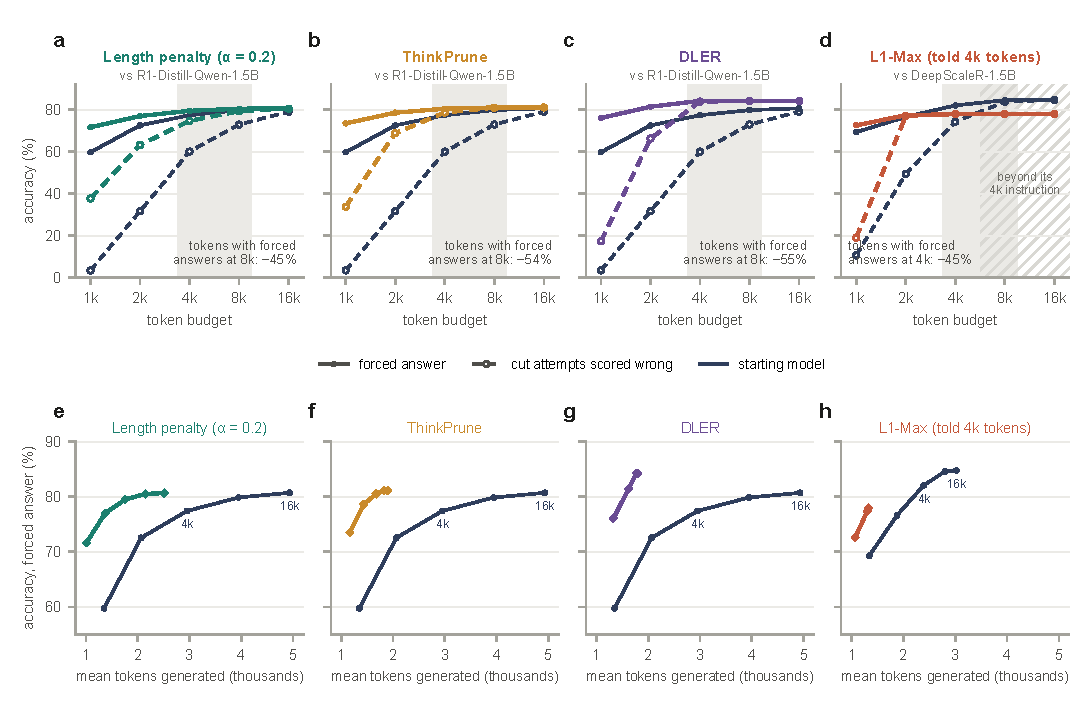
\includegraphics[width=\textwidth]{fig_ext.pdf}
\caption{\textbf{Published length-reduction methods gain mostly by finishing at a fixed budget, and are more accurate at equal spending (pre-registered test).} MATH-500, four samples per problem; each method (colour) against its own starting model (dark blue), at token budgets of 1k to 16k. Dashed, accuracy when an attempt that has not finished by the budget is scored as wrong; solid, accuracy when it is forced to answer at the budget (Methods). Shaded, the pre-registered budgets of 4k and 8k. \textbf{a}, Length penalty with weight $\alpha=0.2$ (Arora and Zanette). \textbf{b}, ThinkPrune. \textbf{c}, DLER. \textbf{d}, L1-Max told a budget of 4{,}096 tokens; hatched, budgets beyond it. Labels give the change in generated tokens, counting the forced answers, at 8k. \textbf{e}--\textbf{h}, The same forced-answer accuracies against the mean tokens generated per attempt, forced answers included; points are the budgets of 1k to 16k (exploratory). Contrasts with confidence intervals in Supplementary Table~\sref{tab:ext}.}
\label{fig:ext}
\end{figure}

\begin{figure}[t]
\centering
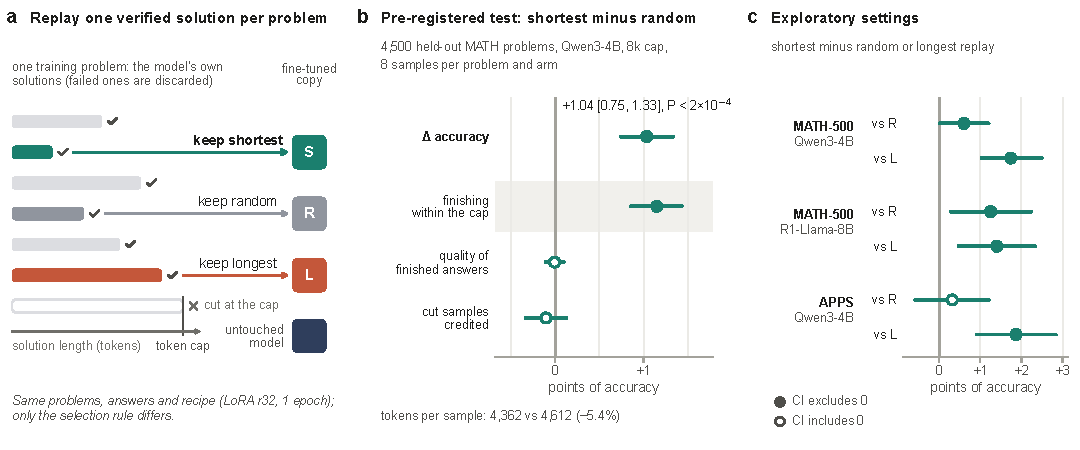
\includegraphics[width=\textwidth]{cover_nc2.pdf}
\caption{\textbf{Replaying the shortest verified solution helps a model finish within its token cap.} \textbf{a}, Identical copies of a model are fine-tuned (LoRA rank 32, one epoch) on one of its own verified solutions per training problem: the shortest (S), a random one (R) or the longest (L); the untouched model is the control. \textbf{b}, Pre-registered test: Qwen3-4B students on the 4,500 MATH test problems outside MATH-500 (8 samples per problem and arm, 8k-token cap). Accuracy of S minus R and its exact split into a finishing term, $\Delta F\,\bar Q$, a quality term, $\Delta Q\,\bar F$, and the share of cut samples that the checker credited (Methods); bars, paired-bootstrap 95\% CIs over problems. \textbf{c}, Shortest minus random and minus longest replay in the exploratory settings (MATH-500 with Qwen3-4B, training run 1 of the three in Table~\ref{tab:rep}, and with R1-Distill-Llama-8B; APPS with Qwen3-4B); dots filled when the interval excludes 0. All $P$ values are two-sided.}
\label{fig:cover}
\end{figure}

\subsection{A controlled experiment: replaying the shortest, a random or the longest verified solution}
To see how the choice of training data acts on finishing, we ran a controlled experiment. In every setting the model first solves training problems several times, each solution is checked by a verifier, and one verified solution per problem is kept for fine-tuning (Fig.~\ref{fig:cover}a). The three training sets contain the same problems and the same correct answers and differ only in the reasoning that precedes the answer. On MATH\cite{hendrycks2021math}, each sample is a single reasoning pass of at most 8k generated tokens, verified against the reference answer; we harvested four samples for each of 2{,}000 training problems, of which the 1{,}345 with at least one verified solution form the training sets, and evaluated on MATH-500\cite{lightman2023verify}, with four samples per problem, and, for the pre-registered test, on the 4{,}500 other problems of the MATH test split (held out from our fine-tuning; like any public benchmark, they may have been seen in pre-training). We used two models from different families, Qwen3-4B-Thinking-2507\cite{qwen3report} and DeepSeek-R1-Distill-Llama-8B\cite{guo2025deepseekr1,grattafiori2024llama3}. On APPS\cite{hendrycks2021apps}, Qwen3-4B writes a program for stdin/stdout problems, verified on hidden tests, under the same cap. We also ran the design on a 27-billion-parameter agent that writes and executes programs for ARC-AGI-2 puzzles\cite{chollet2025arcagi2}, a setting with too few puzzles to resolve the selection contrast, which we report in Supplementary Note~6. Arms are compared with a paired bootstrap over problems; all $P$ values are two-sided (Methods).

\subsection{A pre-registered test: shortest replay beats random replay, by finishing}
On MATH-500 the shortest-replay Qwen3-4B student had beaten the random-replay student by 0.60 points ($P=0.046$), and by 0.95 points over three training runs, but no single shortest-minus-random contrast of the eight in our exploratory settings survived a Holm correction (smallest adjusted $P=0.062$). We therefore asked the question once more, on new problems and with enough samples to answer it. Before any model was evaluated on them, we registered the hypotheses, the 4{,}500 MATH test problems outside MATH-500, the generation settings of the MATH-500 runs (8k cap, temperature 0.6), eight samples per problem and arm, the unchanged students and checker, the test and a stopping rule (Methods; the pre-registration and the hashes of the data and code are released with the paper).

Both hypotheses were supported (Fig.~\ref{fig:cover}b). The shortest-replay model answered 72.76\% of the samples correctly and random replay 71.72\%, a difference of 1.04 points (95\% CI 0.75 to 1.33; paired bootstrap $P<2\times10^{-4}$, sign-flip test $P=10^{-4}$), with no problem excluded. The difference is a finishing difference: shortest replay finished 74.14\% of its samples within the cap, against 72.92\%, and the finishing term of the split is $+1.15$ points (0.86 to 1.43; $P<2\times10^{-4}$); the quality term is $-0.01$ points ($-0.11$ to 0.09; $P=0.89$), and the share of cut samples that the checker credited changes by $-0.11$ points ($P=0.39$). Finished answers were correct 94.27\% and 94.28\% of the time. Shortest replay also generated 5.4\% fewer tokens per sample (4{,}362 against 4{,}612). The effect on the new problems is larger than on MATH-500, and its standard error (0.15 points) is what the pre-registration expected. The test compares one pair of trained models (training run 1): its interval covers problems and sampling, not variation between training runs, which Table~\ref{tab:rep} addresses.

\subsection{The ordering holds across training runs, models and domains}
On MATH-500 the three Qwen3-4B arms are ordered by the length of the replayed solution (Table~\ref{tab:single}): shortest replay reaches 70.02\% accuracy per sample, random replay 69.42\% and longest replay 68.28\%, against 68.93\% for the untouched model. All three independent training runs reproduce the ordering (Table~\ref{tab:rep}); over the three, shortest replay beats random replay by 0.95 points on average ($t$-test with runs as units $P=0.053$) and longest replay by 1.67 ($t$-test $P=0.004$); a hierarchical bootstrap over runs and problems, which with three runs understates the variation between runs, gives 0.27 to 1.72 and 0.99 to 2.39. On R1-Distill-Llama-8B, shortest replay beats random and longest replay by 1.25 and 1.40 points ($P=0.012$ and $P=0.003$) and is neutral relative to the untouched model ($-0.23$; $P=0.64$), whereas random and longest replay harm it ($-1.48$ and $-1.63$ points; $P=0.003$ and $P=0.001$). On APPS no arm improved on the untouched model, but longest replay lowered accuracy by 2.27 points ($P<0.001$) and shortest replay was 1.87 points above longest replay ($P<0.001$; Fig.~\ref{fig:cover}c). At the 8k cap (24k tokens per message for the ARC agent) shortest replay was the cheapest of the three rules in every setting, though by little on APPS ($-0.1\%$ against the untouched model; Supplementary Fig.~\sref{fig:s2}); on AIME at a 32k cap it was not (Supplementary Note~2). On ARC-AGI-2 the agent showed the same direction and the same finishing signature in its message logs, but with 72 puzzles the selection contrast was not resolved (Supplementary Note~6).

On both MATH models the finishing term carries the whole advantage of shortest replay over the other rules (Table~\ref{tab:decomp}): $+1.05$ and $+2.42$ points against random and longest replay on Qwen3-4B, $+1.60$ and $+1.96$ on R1-Llama-8B, all with $P<0.001$, while the quality terms are small and negative ($-0.35$ to $-0.68$).

\subsection{The advantage is not explained by the training dose, the pipeline or sharpening}
Shortest replay trains on fewer tokens than random replay, so its effect could be one of training dose rather than of selection. We built token-matched controls: random and longest replay restricted to the problems of a random permutation, taken in order until their loss tokens matched those of shortest replay (Methods), in two replicates with different permutations. Under an 8k cap (the 32k generations described below, cut samples scored as wrong), shortest replay was ahead of every token-matched arm, significantly in three of four: by 1.95 and 0.68 points against the two token-matched random-replay replicates ($P=0.004$ and $P=0.095$) and by 2.60 and 1.88 points against the two token-matched longest-replay replicates (both $P<0.001$). The token-matched arms also train on fewer problems and optimiser steps. Their two random-replay replicates differed by 2.3 points, but one of them differed by 1.55 points between its own two sampling seeds ($P=0.001$), so we do not read the gap between replicates as an effect of which problems are kept. Keeping every distinct verified solution, the usual practice in rejection-sampling fine-tuning\cite{yuan2023rft}, did no better than random replay and 1.70 points worse than shortest replay at 8k ($P<0.001$). A zero-step adapter run through the same training, merging and saving pipeline left the weights bit-identical to the untouched model and its accuracy at 8k unchanged (Qwen3-4B: $+0.45$ points, $-0.60$ to 1.55, against $+2.20$ for shortest replay on the same sampling seed; R1-Llama-8B, for which the tokenizer needed a workaround: $+0.53$, $P=0.19$). Finally, sampling the untouched model at a lower temperature (0.4 instead of 0.6), a test of the reading that self-training merely sharpens the output distribution, changed neither its accuracy at 8k ($+0.25$ points, $-0.80$ to 1.35) nor its length ($-0.7\%$ tokens at 32k, $P=0.42$); a temperature of 0.4 is a mild probe of this reading.

\begin{table}[t]
\centering\small
\caption{\textbf{Accuracy, finishing and cost in the single-sample settings (exploratory).} Accuracy per sample (\%), mean over seeds; $\Delta$, difference from the untouched model in points, with its paired-bootstrap 95\% CI over the 500 problems and two-sided $P$; finished, share of samples that end within the cap (\%); correct if finished, accuracy divided by the finished share (\%; it includes the cut samples that the checker credited, about 3\% of samples, and so overstates the accuracy of finished answers by about 3--4 points; Methods); tokens, generated tokens per sample. For Qwen3-4B, the replay arms are the first of three training runs (Table~\ref{tab:rep}). Finishing is not reported for APPS (Methods).}
\label{tab:single}
\setlength{\tabcolsep}{5pt}
\begin{tabular}{lcccccc}
\toprule
arm & accuracy & $\Delta$ vs untouched [95\% CI] & $P$ & finished & correct if finished & tokens \\
\midrule
\multicolumn{7}{l}{\textit{MATH-500, Qwen3-4B, 8k cap (5 seeds per arm; round 2, 3 seeds)}} \\
\quad shortest & 70.02 & $+$1.09 [0.50, 1.70] & $<$0.001 & 71.90 & 97.39 & 4{,}442 \\
\quad random & 69.42 & $+$0.49 [$-$0.03, 1.02] & 0.065 & 70.83 & 98.01 & 4{,}694 \\
\quad longest & 68.28 & $-$0.65 [$-$1.36, 0.01] & 0.052 & 69.43 & 98.34 & 5{,}056 \\
\quad untouched & 68.93 & --- & --- & 70.68 & 97.52 & 4{,}708 \\
\quad shortest, round 2 & 71.25 & $+$2.32 [1.55, 3.10] & $<$0.001 & 73.45 & 97.00 & 4{,}230 \\
\multicolumn{7}{l}{\textit{MATH-500, R1-Llama-8B, 8k cap (3 seeds per arm)}} \\
\quad shortest & 80.47 & $-$0.23 [$-$1.22, 0.75] & 0.64 & 87.32 & 92.15 & 3{,}123 \\
\quad random & 79.22 & $-$1.48 [$-$2.48, $-$0.50] & 0.003 & 85.58 & 92.56 & 3{,}322 \\
\quad longest & 79.07 & $-$1.63 [$-$2.63, $-$0.68] & 0.001 & 85.20 & 92.80 & 3{,}515 \\
\quad zero-step (sham) & 81.23 & $+$0.53 [$-$0.28, 1.32] & 0.19 & 87.48 & 92.86 & 3{,}373 \\
\quad untouched & 80.70 & --- & --- & 86.82 & 92.95 & 3{,}413 \\
\multicolumn{7}{l}{\textit{APPS, Qwen3-4B, 8k cap (3 seeds per arm)}} \\
\quad shortest & 36.83 & $-$0.40 [$-$1.43, 0.60] & 0.46 & n/a & n/a & 6{,}834 \\
\quad random & 36.52 & $-$0.72 [$-$1.67, 0.23] & 0.13 & n/a & n/a & 6{,}865 \\
\quad longest & 34.97 & $-$2.27 [$-$3.25, $-$1.33] & $<$0.001 & n/a & n/a & 6{,}924 \\
\quad untouched & 37.23 & --- & --- & n/a & n/a & 6{,}842 \\
\bottomrule
\end{tabular}
\end{table}

\begin{table}[t]
\centering\small
\caption{\textbf{Three independent training runs per replay rule (MATH-500, Qwen3-4B, 8k cap).} Run 1 is the original arms (Tables~\ref{tab:single} and \ref{tab:decomp}); runs 2 and 3 retrain the three arms from the same harvest with other training seeds, which change the data order, the adapter initialisation and the solutions drawn for random replay (Methods). Top: accuracy per sample (\%) and generated tokens per sample, means over sampling seeds. Bottom: differences in points within each run (computed before rounding) and, over the three runs, their mean with the 95\% CI and two-sided $P$ of a hierarchical paired bootstrap that resamples runs and then problems (with three runs it understates the variation between runs), and the two-sided $P$ of a $t$-test on the three run-level differences (two degrees of freedom).}
\label{tab:rep}
\setlength{\tabcolsep}{4pt}
\begin{tabular}{lccccccccc}
\toprule
 & \multicolumn{2}{c}{run 1 (5 seeds)} & \multicolumn{2}{c}{run 2 (2 seeds)} & \multicolumn{2}{c}{run 3 (2 seeds)} & \multicolumn{3}{c}{three runs} \\
\cmidrule(lr){2-3}\cmidrule(lr){4-5}\cmidrule(lr){6-7}\cmidrule(lr){8-10}
arm & accuracy & tokens & accuracy & tokens & accuracy & tokens & mean [95\% CI] & $P$ & $P$, $t$-test \\
\midrule
shortest (S) & 70.02 & 4{,}442 & 70.45 & 4{,}399 & 70.22 & 4{,}390 & & & \\
random (R) & 69.42 & 4{,}694 & 69.08 & 4{,}713 & 69.35 & 4{,}639 & & & \\
longest (L) & 68.28 & 5{,}056 & 68.97 & 5{,}056 & 68.42 & 5{,}040 & & & \\
\midrule
S $-$ R & $+$0.60 & & $+$1.38 & & $+$0.88 & & $+$0.95 [0.27, 1.72] & 0.007 & 0.053 \\
S $-$ L & $+$1.74 & & $+$1.48 & & $+$1.80 & & $+$1.67 [0.99, 2.39] & $<$0.001 & 0.004 \\
R $-$ L & $+$1.14 & & $+$0.10 & & $+$0.93 & & $+$0.72 [$-$0.10, 1.49] & 0.077 & 0.15 \\
\bottomrule
\end{tabular}
\end{table}

\begin{table}[t]
\centering\small
\caption{\textbf{The advantage of shortest replay, split into finishing and quality (MATH-500, 8k cap, exploratory).} Accuracy difference (points) between shortest replay and the arm named, and its split into a finishing term, $\Delta F\,\bar{Q}$, and a quality term, $\Delta Q\,\bar{F}$, with $Q=A/F$ (Methods); paired-bootstrap 95\% CIs over the 500 problems; two-sided $P$ (for each term, that of $\Delta F$ or $\Delta Q$). The terms add up to the accuracy difference up to rounding. Because $Q=A/F$ here includes the cut samples that the checker credited, the quality term also absorbs changes in their share, which may explain the small negative quality terms; the pre-registered split, which separates them, has a quality term of $-0.01$ points. Qwen3-4B arms: run 1 of Table~\ref{tab:rep}. The pre-registered split on 4{,}500 new problems is in Fig.~\ref{fig:cover}b.}
\label{tab:decomp}
\setlength{\tabcolsep}{4.5pt}
\begin{tabular}{lcccccc}
\toprule
shortest replay & $\Delta$ accuracy [95\% CI] & $P$ & finishing term [95\% CI] & $P$ & quality term [95\% CI] & $P$ \\
\midrule
\multicolumn{7}{l}{\textit{Qwen3-4B}} \\
\quad vs random & $+$0.60 [0.01, 1.20] & 0.046 & $+$1.05 [0.52, 1.61] & $<$0.001 & $-$0.45 [$-$0.94, 0.05] & 0.080 \\
\quad vs longest & $+$1.74 [1.03, 2.49] & $<$0.001 & $+$2.42 [1.60, 3.31] & $<$0.001 & $-$0.68 [$-$1.33, $-$0.07] & 0.028 \\
\quad vs untouched & $+$1.09 [0.50, 1.70] & $<$0.001 & $+$1.19 [0.59, 1.81] & $<$0.001 & $-$0.10 [$-$0.58, 0.40] & 0.68 \\
\multicolumn{7}{l}{\textit{R1-Llama-8B}} \\
\quad vs random & $+$1.25 [0.28, 2.23] & 0.012 & $+$1.60 [0.80, 2.43] & $<$0.001 & $-$0.35 [$-$0.94, 0.23] & 0.23 \\
\quad vs longest & $+$1.40 [0.47, 2.33] & 0.003 & $+$1.96 [1.16, 2.76] & $<$0.001 & $-$0.56 [$-$1.16, 0.03] & 0.060 \\
\quad vs untouched & $-$0.23 [$-$1.22, 0.75] & 0.64 & $+$0.46 [$-$0.39, 1.30] & 0.28 & $-$0.70 [$-$1.37, $-$0.03] & 0.039 \\
\bottomrule
\end{tabular}
\end{table}

\subsection{A restart view of the token cap}
Why should the length of a replayed solution matter, when all three training sets contain the same problems and the same answers? Let $L$ be the number of tokens an attempt needs to reach its answer under a cap $t$. The attempt finishes when $L\le t$; otherwise it is cut, and scored as wrong or, in an agent, discarded before the next message starts again. Accuracy per attempt factorises as
\begin{equation}
A(t)=F(t)\,Q(t),\qquad F(t)=P(L\le t),
\label{eq:fq}
\end{equation}
where $Q(t)$ is the probability that a finished answer is correct. A split of this kind has been used to describe reasoning efficiency\cite{kaiser2026decomposing,nie2026truncation}; we use it to state what a shift in length implies. On MATH it is the cap, not the answers, that limits accuracy: scored at 8k tokens, 29.8\% of the untouched Qwen3-4B's samples are cut (2.8\% cut but credited by the checker), whereas 4.3\% finish with a wrong answer (32k generations, below). When a cut attempt is followed by a fresh one, attempts under a cap form a restart strategy with a fixed cutoff\cite{luby1993optimal}, whose expected cost per finished attempt is
\begin{equation}
C(t)=\frac{\E[\min(L,t)]}{P(L\le t)}.
\label{eq:restart}
\end{equation}
If fine-tuning on short solutions makes $L$ stochastically shorter without changing which answers the model can reach, then at every cap $F(t)$ can only rise and $\E[\min(L,t)]$ can only fall, so the shorter policy is never more expensive per finished attempt, while the accuracy it gains is at most $Q(t)\,[1-F(t)]$. The view makes three predictions, which we did not pre-register: at a binding cap, the advantage of shortest replay lies in $F$, not in $Q$ (tested above); when the cap is loosened, the advantage shrinks and finishing rates converge; and shortest replay stays cheaper. An alternative, in which short solutions teach the task better because they contain fewer wrong steps to imitate, would show up as a gain in $Q$ that persists at a looser cap; the two accounts are not exclusive.

\begin{figure}[t]
\centering
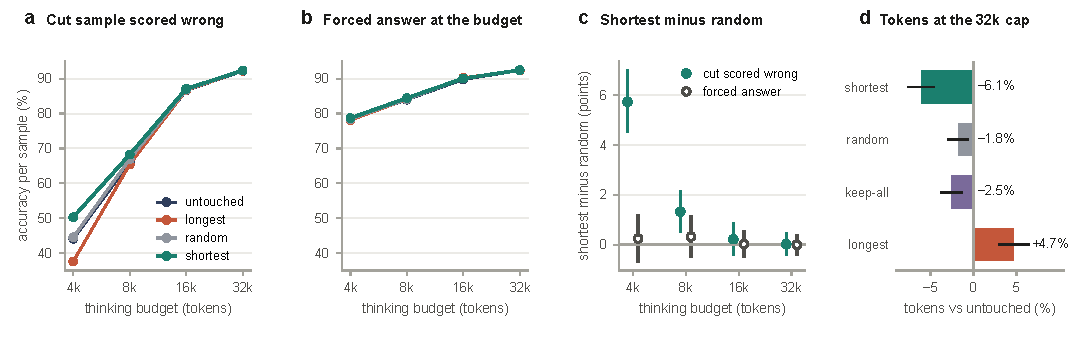
\includegraphics[width=\textwidth]{fig_cap.pdf}
\caption{\textbf{The advantage tracks the cap; with forced answers the arms differ little in accuracy and shortest replay is cheaper.} MATH-500, Qwen3-4B, generations with a 32k-token cap (two sampling seeds per arm, four samples per problem), scored at thinking budgets $t$ of 4k, 8k, 16k and 32k tokens. \textbf{a}, Accuracy when a sample that has not finished by $t$ is scored as wrong, for the untouched model and the three replay rules. \textbf{b}, Accuracy when a sample that has not finished by $t$ is closed with the model's thinking-budget instruction and forced to answer (Methods). \textbf{c}, Shortest replay minus random replay under the two scorings; bars, paired-bootstrap 95\% CIs over the 500 problems. \textbf{d}, Generated tokens per sample at the 32k cap, change relative to the untouched model.}
\label{fig:cap}
\end{figure}

\subsection{Loosening the cap removes the advantage but not the brevity}
We generated every Qwen3-4B arm on MATH-500 again with a 32k-token cap, the output length the model card recommends for most queries (it recommends 81{,}920 tokens for competition-level problems), with two sampling seeds, and scored the same generations as if the cap had been 4k, 8k, 16k or 32k (Fig.~\ref{fig:cap}a; Methods). At 32k fewer than 1\% of the samples are cut and accuracy differs by less than half a point between arms (91.95--92.42\%, controls included; shortest minus untouched $+0.12$ points, $-0.45$ to 0.70; Supplementary Table~\sref{tab:s32k}). The advantage of shortest replay over random replay falls as the cap is loosened, from $+5.72$ points at 4k (4.55 to 6.97), $+1.32$ at 8k (0.53 to 2.13), $+0.23$ at 16k ($-0.40$ to 0.85) and $+0.03$ at 32k ($-0.38$ to 0.42; within $\pm0.5$ points by two one-sided tests), with cut samples scored as wrong; with the checker's credit for cut samples, as in Tables~\ref{tab:single} and \ref{tab:decomp}, the same contrasts are $+4.72$, $+0.75$, $+0.22$ and $+0.02$ points. Against longest replay, $+12.68$, $+2.83$, $+0.33$ and $+0.10$ points. An earlier, independent evaluation at 8k and 16k with separate generations had shown the same: shortest minus longest replay fell from $+1.74$ to $+0.17$ points (change $+1.56$, $P<0.001$). Shortest replay nevertheless stayed the cheapest arm at 32k, with 6.1\% fewer tokens per sample than the untouched model ($-7.5$ to $-4.7\%$), 4.3\% fewer than random replay and 10.3\% fewer than longest replay (all $P<0.001$; Fig.~\ref{fig:cap}d). The shift in length is concentrated in short attempts: by 4k tokens shortest replay had finished 53.3\% of its samples and the untouched model 47.1\%, by 16k both 92.7\%; the median finished length fell from 4{,}550 to 3{,}368 tokens, while the 90th percentile barely moved (14{,}190 against 14{,}590). Loosening the cap removed the gain but not the brevity, consistent with a shift in length rather than in answer quality; a per-problem check agrees (Supplementary Note~3).

\subsection{A forced answer at the cap recovers most of the gain}
The restart view also says what the gain is worth. If shortest replay helps by letting more attempts finish, any other way of making attempts finish should give the same gain. Qwen3-4B supports such a way at inference: when the thinking budget runs out, the reasoning is closed with a fixed instruction and the model is asked to answer\cite{qwen3report,muennighoff2025s1}. We applied it to the saved generations of every arm at each budget (Fig.~\ref{fig:cap}b). With forced answers, on MATH-500 no arm differed significantly from another at any budget (78.1--78.9\% at 4k and 84.0--84.5\% at 8k, controls included): shortest minus random replay was $+0.25$ points at 4k ($-0.65$ to 1.15), $+0.33$ at 8k ($-0.47$ to 1.12) and $+0.03$ at 16k, and shortest replay minus the untouched model $+0.00$, $+0.47$ and $+0.28$ points (none significant; Fig.~\ref{fig:cap}c); with upper bounds near 1 point at 4k and 8k, a residual difference of that size is not excluded. A forced answer at 8k is worth 18 points to the untouched model, against 2.3 points for shortest replay without forcing (both with cut samples scored as wrong). What it adds under forcing is mainly cost: it reaches about the same accuracy with fewer generated tokens, counting the forced answers. Per sample, shortest replay generated 5.5\% fewer tokens than the untouched model at 4k ($-6.5$ to $-4.5\%$), 6.5\% fewer at 8k ($-7.7$ to $-5.4\%$) and 6.3\% fewer at 16k ($-7.5$ to $-5.1\%$), and 5.0\%, 6.0\% and 5.1\% fewer than random replay (all $P<0.001$), the same saving as at the 32k cap. Random replay saved at most 1.2\% against the untouched model at these budgets, and longest replay cost 5--7\% more.

The intervals on MATH-500 left room for a residual difference of about 1 point, the size of the pre-registered effect. We therefore forced answers on the saved generations of the pre-registered test, at 4k and 8k tokens, in a pre-registered amendment (Methods). The forced answer removed most of the advantage of shortest replay but not all of it. At 8k, shortest minus random replay fell from 1.04 points with the pre-registered scoring to 0.34 points with forced answers (0.09 to 0.60), a reduction of 0.69 points ($-1.04$ to $-0.36$; $P<2\times10^{-4}$); at 4k it fell from 4.26 to 0.53 points (0.25 to 0.81). We had predicted that the forced difference would lie within $\pm0.5$ points; its 90\% interval, 0.13 to 0.56, does not. The prediction ignored that a policy that progresses faster is further along when it is cut: the residual is close to what a descriptive model of 5\% faster progress gives (0.40 points at 8k; Supplementary Note~8), so it need not be a gain in the answers. The pre-registered split and the forced answer measure different things: the split puts the whole difference in finishing because finished answers were equally often correct, and forcing removes two-thirds of it. It also kept its lower cost: with forced answers it generated 5.4\% fewer tokens than random replay at 8k ($-5.7$ to $-5.0\%$) and 4.5\% fewer at 4k (Supplementary Table~\sref{tab:amend}).

\section{Discussion}
Does shorter reasoning mean better reasoning? Mostly not: it means reaching the answer sooner. Under a tight token limit, shorter reasoning lets more attempts finish, and at our pre-registered limits this carried most of the gain: a forced answer from the starting model recovered 10.7 of the 13.8 points that three published methods gained, and two-thirds of the advantage of our controlled replay rule. What survived a forced answer was, except for DLER, close to a descriptive model of faster progress (Supplementary Note~8), not a causal attribution. DLER kept 3.5 to 4.4 points, close to what reinforcement learning gave DeepScaleR from the same starting model, so its gain more likely comes from the training than from brevity. Shorter reasoning also costs less, an advantage in itself for a service paying for tokens: at equal average spending three methods were more accurate than their starting model (Fig.~\ref{fig:ext}e--g; exploratory). These contributions, finishing, speed and cost, change weight with the limit (Fig.~\ref{fig:concept}c--g). Chess engines are tested with the same distinction: a change that only speeds up search wins games under a clock but not at a fixed search depth. Scoring cut attempts as wrong, or forcing an answer at a tight limit, is a test under a clock; a loose limit is the test at fixed depth, and there the gains of shortening vanished. Crediting a gain to better reasoning requires that test, and crediting it all to the limit misses speed and cost.

Among a model's own verified solutions, the shortest is the best of three replay rules under a binding cap: it beat random replay in a pre-registered test on 4{,}500 new problems, and in exploratory settings the ordering shortest $>$ random $>$ longest held, in point estimates, across three training runs, two model families and programming. We found no evidence that the gain reflects training dose, the fine-tuning pipeline or a sharper output distribution. In the pre-registered test and in every MATH comparison the finishing term carried the effect and finished answers were no better, matching recent observations that concise reasoning helps by finishing before the deadline\cite{carlon2026shorter}.

The restart view predicts two further properties of this gain, and our exploratory data are consistent with both. First, the advantage appears where the cap binds: it shrank from 5.7 points at 4k to zero at 32k, where shortest replay remained 4--6\% cheaper on MATH. The share of attempts cut at the deployment cap therefore bounds, before any training, how much length-based selection can raise accuracy when cut attempts are lost: at 8k about 27\% of the untouched Qwen3-4B's samples are cut and not credited, out of 31.1 points of error, against at most 13.2\% of R1-Llama-8B's (19.3 points of error), and shortest replay improved on the untouched model only for the first. Second, any other way of finishing should give the same answers: a forced answer at the cap raises every arm far more than training does (18 points for the untouched model at 8k, against about 2 for shortest replay without forcing) and leaves at most a small difference between arms (0.34 points on 4{,}500 problems). The two combine rather than compete: with forced answers, shortest replay is slightly more accurate than random replay and generates 5--6\% fewer tokens, and about 6\% fewer than the untouched model on MATH-500. These properties reconcile our result with reports that shortest-solution fine-tuning hurts at long budgets\cite{arora2025training}: at a budget that does not bind, the view predicts no gain and leaves room for a loss in $Q$.

The practical message is specific. Pipelines that keep every verified solution, or a random one\cite{zelikman2022star,yuan2023rft,gulcehre2023rest}, can choose the shortest at no cost whenever a problem has more than one verified solution (92\% of our MATH training problems), and under a cap this yields a policy that finishes more often, on MATH generates 5--9\% fewer tokens with or without forced answers, and was never significantly less accurate than the untouched model in our settings. The saving is not universal: on APPS it was negligible, and on AIME at 32k, where attempts are long, shortest replay was not shorter. Where accuracy under a cap is the goal, a forced answer should be the baseline against which any training intervention is compared, and evaluations of length-reducing methods should report the cap, the finishing rate and whether cut attempts were rescued; scoring every cut sample as wrong maximises the apparent benefit of brevity. Such reporting is still uncommon among training methods. Of 13 training-based length-reduction methods described in a 2025 survey\cite{sui2025stopoverthinking}, none reports the share of samples cut at the evaluation cap and one compares an answer forced at it, while 11 report an accuracy gain over their starting model or a trained baseline in at least one setting (Supplementary Note~4). Our test of published methods shows what such reporting changes: their accuracy gains at a fixed budget were mostly gains in finishing, which a forced answer delivers without training, while their savings in tokens were real; DLER showed that the comparison can also reveal a gain in the answers, here from reinforcement learning. The one published forced-answer comparison reported L1 far ahead of budget forcing at 512 and 1{,}024 tokens\cite{aggarwal2025l1}; at 1{,}024 tokens our forced starting model was not behind L1-Max, though with more tokens counted (Supplementary Table~\sref{tab:ext}). Where forcing suffices and where training is needed is therefore a question of measurement, and the cut share and a forced baseline are what answer it.

Why the shortest solutions shift the length distribution without degrading the answers (earlier commitment, fewer verification loops) remains untested.

Our study has limitations. The pre-registered replay test and its amendment cover one model, one domain, one cap and one pair of trained models; apart from the pre-registered tests, everything else, including the comparisons at equal spending, is exploratory. We repeated training three times only for Qwen3-4B on MATH; other settings use one fine-tuned model per arm. The 32k and forced-answer analyses use one training run of each arm, two sampling seeds (one for the token-matched, zero-step and temperature controls) and one forcing instruction, Qwen's own; sampling seeds alone moved one model by 1.55 points at 8k. The Qwen3-4B fine-tuning contexts carried a system prompt left over from the ARC agent, absent at evaluation, for every arm (Methods). The pre-registered and the exploratory MATH scoring credit a cut sample whose reasoning already contains a boxed answer (about 3\% of samples; Methods), which the split reports separately. Our amendment's prediction that a forced answer would leave no difference between shortest and random replay failed. Forced answers add up to about 1{,}050 tokens beyond the budget, so accuracy at a nominal budget is not matched in compute; the token counts include them. The speed-only predictions are exploratory, assume that a method runs its starting model's reasoning faster by the ratio of median lengths, and were made after the data were seen. On ARC-AGI-2 the selection contrast is not resolved, and the agent's gain over the untouched model is not significant when seeds are the unit ($P=0.15$). We used one fine-tuning recipe (LoRA rank 32, one epoch). The per-problem length check was defined after the cap data were seen and is informative on few problems. The test of published methods covers one benchmark, models of 1.5 billion parameters, one sampling seed and Qwen's forcing instruction rather than each method's own; its per-problem length check, listed as exploratory in its pre-registration, was not run. The literature audit covers the methods of one 2025 survey and records what the papers report, not whether their gains are gains in finishing.

\section{Methods}
\paragraph{Models.} The single-sample settings use Qwen3-4B-Thinking-2507 (\texttt{Qwen/Qwen3-4B-Thinking-2507}; MATH and APPS) and DeepSeek-R1-Distill-Llama-8B\cite{guo2025deepseekr1} (MATH). The ARC agent is Qwen3.8-27B\cite{qwen38card} in bfloat16. All generation uses vLLM\cite{kwon2023vllm}.

\paragraph{Training sets and fine-tuning.} Per problem, S keeps the verified solution with the fewest generated tokens, R one drawn uniformly at random with a fixed seed, and L the one with the most. MATH: 2{,}000 training problems drawn with seed 0 from the 5{,}582 training problems of levels 3--5, four samples each at the 8k cap; 1{,}345 had at least one verified solution and form the training sets (1{,}235 with at least two distinct ones), and the replayed solutions average 3{,}588 (S), 4{,}397 (R) and 5{,}272 (L) tokens; the verifier is a normalised match of the last \texttt{\textbackslash boxed\{\}} expression. APPS: 2{,}000 training problems with stdin/stdout tests; a solution is verified when its last Python block passes up to ten tests, 4~s each; 765 training problems had a verified solution. Fine-tuning: LoRA\cite{hu2022lora} rank 32, $\alpha=64$, AdamW ($\beta$ 0.9, 0.99), learning rate $5\times10^{-5}$ with 20 warm-up steps and cosine decay, one epoch, effective batch 8, maximum length 12{,}288 tokens, loss on the assistant tokens with the reasoning included; each example's loss is the mean over its own target tokens, so every example has the same weight whatever its length; adapters merged for evaluation. In the single-sample settings S, R and L therefore have the same number of examples and optimiser steps (169 for Qwen3-4B on MATH, 217 for R1-Llama-8B, 96 on APPS) and differ in loss tokens; on ARC-AGI-2, where examples longer than the maximum length are skipped, the three arms took 72, 68 and 63 steps. For Qwen3-4B, the fine-tuning context of every MATH and APPS example began with the ARC agent's system prompt (``You are an expert at solving ARC (Abstraction and Reasoning Corpus) puzzles by writing Python.''), a leftover of the shared training script; evaluation used no system prompt, and all arms and controls share this context. R1-Llama-8B: the same protocol, with no system prompt in the fine-tuning data; its tokenizer had to be loaded as \texttt{PreTrainedTokenizerFast} to work around a tokenizer-loading bug in version~5 of the transformers library. Training replicates: for Qwen3-4B on MATH, the three arms were trained twice more with training seeds 1 and 2, which set the data order, the adapter initialisation and, for R, the drawn solutions.

\paragraph{Controls.} Keep-all: every distinct verified solution of every problem (duplicates removed after whitespace normalisation). Token-matched (Rtm, Ltm): R and L restricted to the problems of a fixed random permutation, taken in order until their loss tokens reached those of S; two replicates with permutation seeds 20261102 and 20261120. They match S in loss tokens and have fewer examples and steps. Zero-step (sham): the S training set trained with learning rate 0 for one step (PEFT initialises the LoRA up-projection to zero) and merged and saved by the same pipeline; a check confirmed that all weight tensors are bit-identical to the untouched model and that the saved configuration differs only in the field layout written by version~5 of the transformers library, with the same values. Lower temperature: the untouched model sampled at 0.4 instead of 0.6.

\paragraph{Evaluation and scoring (MATH, APPS).} Temperature 0.6, top-$p$ 0.95, top-$k$ 20, four samples per problem per seed, no system prompt. At the 8k cap the paper's checker scores a sample by the last \texttt{\textbackslash boxed\{\}} of its answer or, for a sample cut at the cap, of its reasoning; a cut sample is therefore credited when its reasoning already contains the right boxed answer (2.9\% of samples in the pre-registered test). A sample is \emph{finished} when it ends within the cap. For two arms $a$ and $b$, with $F$ the finished share, $Q$ the share correct among finished samples and $C$ the share of samples cut but credited, $A=FQ+C$ and $A_a-A_b=(F_a-F_b)(Q_a+Q_b)/2+(Q_a-Q_b)(F_a+F_b)/2+(C_a-C_b)$ exactly. The pre-registered analysis reports the three terms; the exploratory MATH-500 tables report $Q=A/F$, which includes $C$. On APPS the cut flag also counted samples without a code block, so finishing is not reported there.

\paragraph{Pre-registered test.} The pre-registration (written and hashed on 2026-11-19, before any model was evaluated on these problems) fixed: the problems, the MATH test split (EleutherAI/hendrycks\_math, seven subjects) minus the 500 problems of MATH-500 matched on whitespace-normalised text, 4{,}500 problems, all with a boxed reference answer; the students \texttt{math4b\_S} and \texttt{math4b\_R} of training run 1, unchanged; the 8k generation settings above with sampling seeds 0 and 1 (eight samples per problem and arm); the checker; H1, accuracy per sample of S greater than that of R, tested with a two-sided paired bootstrap over problems ($B=10{,}000$, seed 0, $P=2\min$ of the shares of resampled differences $\le0$ and $\ge0$) with a paired sign-flip test reported alongside; H2, conditional on H1, that the finishing term's interval lies above 0 and the quality term's estimate is at most 0; and a stopping rule (both arms on both seeds to completion; the difference not computed before all four runs were complete). All four runs completed with no missing problem. Deviations from the pre-registration: (i) the evaluation driver printed each run's overall accuracy as it finished (S seed 0, R seed 0, S seed 1, R seed 1), so a partial difference was visible before all four runs were complete, against the intent of the stopping rule; no run was stopped or changed; (ii) the analysis script was written after the runs had finished, before the difference was computed; (iii) the pre-registration calls the split per-problem ``as in the paper''; as in the paper's tables, the analysis computes it from shares pooled over problems, with problems resampled; (iv) the pre-registration said that it and the preparation and launch scripts would be committed to git before the first evaluation job; no commit was made. Instead, the SHA-256 hashes of the pre-registration (\texttt{e1f37784\ldots f15afef}), the problem file and the preparation, launch and generation scripts were written to a log with a timestamp, 2026-11-19 10:12:36 UTC, before the first evaluation job was submitted to the computing centre's scheduler at 10:22:38 UTC (a smoke job submitted at 10:12:56 UTC was cancelled after 9~s, before evaluating any problem). The timestamp in the log is written by us; the submission times are recorded by the computing centre. The pre-registration, the log with its full hashes, the scheduler records and the hashes of the analysis script and its output are released.

\paragraph{Amendment: forced answers in the pre-registered test.} An amendment to the pre-registration, written on 2026-11-24 after the test had been reported and before any forced answer was produced on these generations, fixed: forced answers on the saved generations of the four pre-registered runs at budgets of 4{,}096 and 8{,}192 tokens with the procedure below, each student forcing its own samples; H3, that at 8k the shortest-minus-random difference is smaller with forced answers than with the pre-registered scoring (per problem, the difference of the two differences, bootstrapped as below); H4, that at 8k the forced difference is equivalent to zero within $\pm0.5$ points (90\% bootstrap interval inside the margin); and the secondary analyses. The amendment states what was known when it was written. Its hash, with those of the analysis, forcing and launch scripts and the problem file, was logged at 2026-11-24 19:31:11 UTC, before the first forcing job was submitted. All four runs completed at both budgets, with no problem excluded; the hash of the analysis script was checked before it was run. H3 was supported and H4 was not.

\paragraph{Cap and forced-answer analyses.} Every Qwen3-4B arm was generated on MATH-500 with max\_tokens 32{,}768 (context 34{,}816), otherwise as above, with sampling seeds 0 and 1 (untouched, S, R, L, keep-all) or 0 (controls; the token-matched arms also with seed 1 for the first replicate). At a budget $t$, a sample that ended by itself within $t$ tokens keeps its correctness; for the cut-as-wrong scoring, any other sample is wrong; for the forced scoring, its first $t$ tokens are kept, the reasoning is closed with Qwen's thinking-budget instruction (``Considering the limited time by the user, I have to give the solution based on the thinking directly now.'' followed by the end-of-reasoning token) and the model writes at most 1{,}024 answer tokens with the same sampling settings, scored by the same checker. A sample that had already closed its reasoning within its first $t$ tokens is continued without the instruction. Tokens under forcing count, per sample, the generated tokens of a sample that ended within $t$, and otherwise the $t$ kept tokens, the 25 tokens of the instruction (when added) and the answer tokens written. The independent 8k and 16k evaluations of the earlier MATH-500 cap test used separate generations with those caps (two seeds per arm at 16k).

\paragraph{Length-only prediction.} For a trained arm $X$ and a reference arm $Y$ (the untouched model unless stated) on the 32k generations, the samples of each arm on a problem (both sampling seeds pooled) are ranked by length, samples unfinished at 32k last. At budget $t$, the $k$-th shortest sample of $X$ is predicted correct if the $k$-th shortest sample of $Y$ is finished and correct and the $X$ sample has at most $t$ tokens; cut samples are scored as wrong. The prediction uses the lengths of $X$ but not its correctness. Controls replace the ranked correctness of $Y$ by the same values shuffled within the problem, by $Y$'s per-problem share correct among finished samples $q_i$, which gives $\hat A_X(t)=N^{-1}\sum_i q_i F_i^X(t)$ with $F_i^X(t)$ the share of $X$'s samples on problem $i$ finished by $t$, or by one share for all problems. Calibration contrasts, in which answer quality cannot have changed, predict the zero-step adapter and the lower temperature from the untouched model on seed 0, and each seed of the untouched model from the other. The residual, observed minus predicted accuracy, is bootstrapped over problems as below (script \texttt{synth/natcomm\_length\_predict.py}).

\paragraph{Published methods (pre-registered test).} The pre-registration (written on 2026-11-22 before any of these models was evaluated by us) fixed the models, the settings, the hypothesis, the analysis script and a stopping rule; the SHA-256 hashes of the pre-registration (\texttt{a1758c70\ldots efc65723}), the analysis, generation, forcing and launch scripts and the problem file were written to a log at 2026-11-22 18:16:21 UTC, and the first evaluation job was submitted to the scheduler at 18:16:28 UTC. Models (HuggingFace main branch, revisions in Supplementary Note~5): DeepSeek-R1-Distill-Qwen-1.5B; the Arora--Zanette models trained from it with length-penalty weights $\alpha=0$ and $0.2$; ThinkPrune (iterative pruning to 2k tokens); DLER (research checkpoint); DeepScaleR-1.5B-Preview; L1-Qwen-1.5B-Max. All weights in bfloat16 (four checkpoints are stored in float32). MATH-500, four samples per problem, sampling seed 0, temperature 0.6, top-$p$ 0.95, no top-$k$ (the settings recommended for R1-Distill), max\_tokens 16{,}384, each model's own chat template with the generation prompt ending in the opening reasoning tag and a single beginning-of-sequence token. Prompts: the paper's for the R1-Distill models; DeepScaleR's training prompt (``Let's think step by step and output the final answer within \texttt{\textbackslash boxed\{\}}.'') for DeepScaleR and L1-Max, with ``Think for maximum $N$ tokens.'' appended for L1-Max ($N=4{,}096$ for the primary arm, 1{,}024 for an exploratory one). Forced answers at budgets of 1k, 2k, 4k, 8k and 16k tokens as above, with Qwen's instruction (24 tokens under these models' tokenizer). Primary statistic: per problem, the mean over the four method contrasts and the budgets 4k and 8k of [forced gain $-$ cut-as-wrong gain], bootstrapped over problems as below; H1, a negative mean with $P<0.05$. The cost calibration on the first model exceeded the pre-registered 30 CPU-hours (32.9); as pre-registered, the author decided to continue before anything else was submitted. The launcher printed each run's overall accuracy as it finished, as the pre-registration allows; no contrast was computed before all runs and forced answers were complete. The per-problem length check, listed as exploratory, was not run. All eight runs completed with no missing problem (the two evaluation shards of the first model reached their wall-time limit after writing all their problems and are recorded by the scheduler as timed out); the hash of the analysis script was checked before it was run. The pre-registration describes the test as an exploratory extension of this paper; its hypothesis, statistic and analysis were fixed before any evaluation, and we report it as a pre-registered test.

\paragraph{ARC-AGI-2 agent.} Temperature 1.0, top-$p$ 0.95, top-$k$ 20, reasoning enabled. In each message the model writes one Python block, either an exploratory program, whose printed output is returned, or a submission defining a \texttt{transform} function, which runs on every training input and returns per-pair feedback. At most six messages of 24{,}000 generated tokens each within a context of 98{,}304 tokens. A message that reaches the limit without closing its reasoning is cut: its reasoning is not kept, and the next user message asks for one Python block. A trajectory is verified when its final program reproduces all training outputs and the test output. Verified trajectories were harvested on ARC-AGI-2 training puzzles, public-evaluation puzzles outside the evaluation set and synthetic puzzles; puzzles whose shortest verified trajectory exceeds 15{,}000 tokens were dropped from all arms, and every puzzle seeded from an evaluation puzzle was removed (387 puzzles). Each trajectory is split into one training example per assistant message. The 72 evaluation puzzles (40 development puzzles and 32 untouched by any harvest) are excluded from training; five seeds per arm; a puzzle is solved when, for every test input, one of two submitted outputs is exact. The ARC-AGI-2 results, without the analyses of this paper's MATH experiments, were submitted as a write-up to the ARC Prize 2026 paper track (Kaggle, November 2026).

\paragraph{Statistics.} Comparisons between arms are paired over problems (puzzles for ARC). Per problem we average the outcome over samples and seeds; the difference between two arms is the mean over problems, in percentage points (puzzles of 72 for ARC). We resample problems with replacement 10{,}000 times\cite{efron1993bootstrap}; the 95\% CI is the 2.5th and 97.5th percentiles; with $p$ the share of resampled differences $\le0$, $P=2\min(p,1-p)$, and values below the bootstrap's resolution are reported as $P<2\times10^{-4}$ or $P<0.001$. Equivalence at 32k is tested with two one-sided tests, a 90\% bootstrap interval inside $\pm0.5$ points. Relative changes in tokens are ratios of total tokens, bootstrapped likewise. For training replicates, a hierarchical bootstrap resamples runs and then problems, and a $t$-test takes runs as units. Apart from the two pre-registered tests and the amendment, all analyses are exploratory; we report Holm-adjusted $P$ values for the eight selection contrasts of the exploratory settings in Supplementary Note~1, together with a test pooled over settings. For ARC-AGI-2, an exact permutation test on the five seed totals per arm takes seeds as the unit.

\paragraph{Use of large language models.} Claude (Anthropic; Claude Opus models, 2026) was used under the author's direction to write and review code for the experiments, the job management on the computing cluster, the statistical analyses and the figures; to search and check the literature; and to draft and edit text from the author's results and instructions. The author designed the study and the pre-registration, decided every analysis and interpretation, checked the code, the numbers and the references, and takes full responsibility for the content. Every number in the paper is regenerated by the released scripts from the released data.

\section*{Data availability}
The summary statistics behind every table and figure, the pre-registrations with their hash logs and the scheduler records are available at \url{https://github.com/cristianocapone/shorter-reasoning}. The per-problem results, the saved generations and the forced answers are available from the author on request. MATH, MATH-500, APPS and ARC-AGI-2 are publicly available.

\section*{Code availability}
The harvesting, selection, fine-tuning, evaluation, forced-answer and statistics code, the launch scripts for the computing cluster, the pre-registrations and the scripts that draw every figure are available at \url{https://github.com/cristianocapone/shorter-reasoning}.

\section*{Acknowledgements}
\begin{sloppypar}
The author acknowledges the CINECA award under the ISCRA initiative (ISCRA Class C project LUCID, HP10CLEJAD) for the availability of high-performance computing resources and support on Leonardo Booster, and the APE Lab, INFN, Sezione di Roma, for access to a server with eight NVIDIA V100 GPUs. This work received no specific funding.
\end{sloppypar}

\section*{Author contributions}
C.C. conceived and designed the study, pre-registered the confirmatory test, directed and verified the code and analyses, and wrote the manuscript with the assistance described in Methods.

\section*{Competing interests}
The author declares no competing interests.

\bibliography{../refs}

\end{document}
